\documentclass{article}
\usepackage[polish]{babel}
\usepackage[T1]{fontenc}
\usepackage{indentfirst}
\usepackage{booktabs}
\usepackage{subfigure}
\usepackage{float}
\usepackage{enumitem}
\usepackage{manyfoot}
\usepackage{caption}


\usepackage[letterpaper,top=2cm,bottom=2cm,left=3cm,right=3cm,marginparwidth=1.75cm]{geometry}

\usepackage{amsmath}
\usepackage{graphicx}
\usepackage[colorlinks=true, allcolors=blue]{hyperref}

\title{Czy na podstawie statystyk meczowych zawodnika możemy przewidzieć jego żółte kartki?}
\author{Adrian Broniecki \\
\small MSiD śr 15:15 TP K01-21c
}

\begin{document}
\maketitle



\section{Wstęp}
Piłka nożna to dynamiczna i emocjonująca gra, w której każdy zawodnik odgrywa istotną rolę w osiągnięciu sukcesu przez swoją drużynę. Jednak oprócz zdolności technicznych i taktycznych, ważnym aspektem gry jest również dyscyplina i fair play na boisku. Jednym z czynników oceniających postawę zawodników jest liczba otrzymanych żółtych kartek.

Ich liczba w piłce nożnej stanowi istotny element oceny i monitorowania zachowań piłkarzy na boisku. Nie tylko wpływa ona na wynik meczu, ale również może mieć konsekwencje dla kolejnych spotkań zawodników, a nawet drużyny jako całości. W tym raporcie przeprowadzę analizę liczby żółtych kartek w zależności od indywidualnych statystyk piłkarzy, aby lepiej zrozumieć czynniki wpływające na ich tendencję do otrzymywania kar.

Celem tej analizy jest uzyskanie głębszego wglądu w związki między poszczególnymi aspektami gry piłkarzy a ich skłonnością do otrzymywania żółtych kartek. Przeanalizuję różne statystyki indywidualne, takie jak liczba fauli, przewinienia, agresywne zachowanie, a także statystyki związane z rolą piłkarza na boisku, takie jak pozycja czy czas gry.

Wyniki tej analizy mogą mieć praktyczne zastosowanie dla trenerów, menedżerów drużyn i sędziów, którzy mogą użyć tych informacji do podejmowania decyzji dotyczących taktyki, selekcji zawodników i oceny ich zachowania na boisku. Ponadto, ta analiza może przyczynić się do zwiększenia świadomości wśród piłkarzy na temat ich własnego zachowania i konsekwencji, które mogą wynikać z otrzymania żółtych kartek.

W kolejnych sekcjach tego raportu przedstawię szczegółowe wyniki analizy oraz wnioski, oraz omówię również ewentualne ograniczenia naszej analizy oraz sugestie dla dalszych badań w tej dziedzinie.

W pracy przedstawię 2 główne próby sprawdzenia, czy liczba zdobytych żółtych kartek przez zawodników w sezonie 2021/2022 jest w jakikolwiek sposób zależna od ich indywidualnych statystyk. Aby to zbadać wykorzystam model regresji, aby móc jak najlepiej przewidzieć wartości dla wszystkich zawodników.




\section{Scrapowanie}
W celu zebrania danych statystycznych dotyczących piłkarzy do analizy, skorzystano z dwóch stron internetowych: \href{https://fbref.com/en/}{fbref.com} oraz \href{https://www.soccerstats247.com/}{soccerstats.com}. Proces zbierania danych został przeprowadzony przy użyciu bibliotek \href{https://pypi.org/project/requests/}{request} oraz \href{https://pypi.org/project/beautifulsoup4/}{BeautifulSoup}.

Głównym celem kodu\footnote{Szczegółowe i opisane kody znajdują się w plikach scraping\_fbref.py oraz scraping\_soccer\_stats.py.} jest scrapowanie danych piłkarzy z różnych lig na podstawie podanych adresów URL i zapisywanie ich w plikach CSV. Umożliwia również określenie różnych wzorców dla różnych typów statystyk, dzięki czemu można łatwo dostosować proces scrapowania do różnych rodzajów danych, takich jak statystyki standardowe lub inne statystyki dodatkowe.

Na stronie \href{https://fbref.com/en/}{fbref.com} dostępny jest szeroki zakres informacji dotyczących statystyk indywidualnych piłkarzy. Zbiór danych zawiera informacje takie jak narodowość, pozycja, wiek, liczba rozegranych meczów, gole, asysty, żółte i czerwone kartki, oraz wiele innych kluczowych wskaźników. Dane te były dostępne dla wielu lig z różnych krajów.

Kolejną stroną, z której pozyskano dane, było \href{https://www.soccerstats247.com/}{soccerstats.com}. Ta strona internetowa również dostarcza szeroką gamę statystyk piłkarskich, takich jak liczba rozegranych meczów, gole, asysty, żółte kartki i wiele innych. Dane te były dostępne dla wielu lig z różnych krajów, co pozwoliło na analizę statystyk piłkarzy na różnych poziomach rozgrywkowych.

Proces scrapowania danych z obu stron internetowych był realizowany zgodnie z zasadami etycznymi i prawnymi, a dane zostały zebrane w sposób zautomatyzowany i precyzyjny.

\section{Zbiory danych i ich przetwarzanie}

\subsection{Wybór danych}
Dane wykorzystane w analizie dotyczą zawodników z TOP 7 najlepszych lig europejskich oraz drugiego stopnia rozgrywkowego w Anglii. Wykorzystane ligi są następujące:

\begin{itemize}
    \item angielska Premier League
    \item włoska Serie A
    \item niemiecka Bundesliga
    \item hiszpańska La Liga
    \item francuska Ligue 1
    \item portugalska Primeira Liga
    \item holenderska Eredivisie
    \item angielskie Championship
\end{itemize}

Powyższe ligi zostały wybrane ze względu na kilka czynników. Pierwszym z nich jest ich poziom sportowy. W tych ligach występują jedne z najlepszych drużyn i piłkarzy na świecie. Zawodnicy grający w tych ligach są często uważani za elitę piłki nożnej, co czyni je interesującymi pod względem analizy ich indywidualnych statystyk. Kolejnym czynnikiem jest różnorodność stylów gry. Każda liga ma swoje charakterystyczne cechy i style gry. Liga angielska jest znana z intensywności i fizyczności, hiszpańska z techniki i umiejętności, a włoska z taktyki i defensywy. Analiza różnic między ligami może ujawnić potencjalne różnice w liczbie żółtych kartek, wynikające z tych różnic w stylach gry. Ostatnim czynnikiem jest popularność i zainteresowanie. Powyższe ligi  cieszą się ogromnym zainteresowaniem zarówno lokalnie, jak i globalnie. Transmisje meczów z udziałem drużyn tych lig są obserwowane przez miliony kibiców na całym świecie. 

\subsection{Zbiory danych}

W pracy zostały wykorzystane 2 zbiory danych:

\begin{enumerate}
    \item Zbiór ”Standards stats” pozyskany ze strony \href{https://fbref.com/en/}{fbref.com}. Zbiór danych zawiera informacje dotyczące piłkarzy, takie jak ich narodowość, pozycja, wiek na początku sezonu oraz różne dane związane z ich występami i osiągnięciami, takie jak liczba meczów rozegranych, gole, asysty, żółte i czerwone kartki. Dodatkowo, zawiera także dane dotyczące oczekiwanych wyników, takie jak spodziewane gole, gole asystowane, oraz informacje dotyczące progresji i wskaźniki na 90 minut. 
    \item Zbiór ”Miscellaneous stats” pozyskany również ze strony \href{https://fbref.com/en/}{fbref.com}. Zbiór danych zawiera wszechstronne informacje dotyczące piłkarzy, ich występów i wyników, takie jak żółte kartki, czerwone kartki, faule, dośrodkowania, przechwyty, wygrane pojedynki powietrzne itp. Jest to kompleksowy zbiór danych umożliwiający analizę indywidualnych statystyk piłkarzy i ich wpływu na liczbę żółtych kartek, które otrzymują.
\end{enumerate}

W ramach scrapowania zebrano dane ze strony \href{https://www.soccerstats247.com/}{soccerstats.com}, lecz okazały się one niewystarczająco obszerne do analizy i ostatecznie nie zostały one wykorzystane.

Powyższe zbiory dla ułatwienia dalszej pracy zostały połączone w jeden zbiór, który później został podzielony na 2 pliki zawierające dane treningowe (statystyki z sezonu 2021/22 dla 8 lig) oraz dane testowe (statystyki z sezonu 2022/23 z angielskiej Premier League i włoskiej Serie A). 
Dla danych ze strony \href{https://fbref.com/en/}{fbref.com}, nazwy nagłówków pozostały bez zmian, zapisane w formie skrótów i w ramach większej czytelności, w plikach \footnote{glossary\_from\_fbref.txt i glossary\_from\_fbref\_miscellaneous.txt} projektu znajdują się rozwinięcia skrótów i ich krótkie opisy.


\subsection{Wstępne przetwarzanie danych}

Obróbka danych zawodników została przeniesiona poza głównego notebook’a i kod przetwarzający dane znajduje się w pliku fbref\_data\_processing.py, gdzie zostały wytłumaczone kolejne czynności przetwarzające dane.

Ze zbiorów zostały odrzuceni zawodnicy, którzy nie rozegrali przynajmniej 3 pełnych meczów (atrybut ‘90s’ $ \geq $ 3.0). Powodem tego jest to, aby wyniki były bardziej rzetelne, gdyż zawodnicy grający mało  zazwyczaj wchodzą z ławki na ostatnie minuty meczu, gdy już sama dynamika gry jest zdecydowanie mniejsza i poszczególne statystyki mogą odbiegać od tych normalnych. Takie przefiltrowanie piłkarzy praktycznie całkowicie rozwiązało problem wybrakowanych lub pustych danych.
Na wszelki wypadek dane zostały jeszcze przefiltrowane i w przypadku niepełnych danych, wiersz był odrzucany.

Ponadto kod łączy moje dwa zbiory - Standard i Miscellaneous Stats – w jeden wspólny zbiór, niezawierający zdublowanych kolumn atrybutów oraz statystyk, które z góry przyjąłem za niepotrzebne tj. gole i asysty oczekiwane itd. Usunięta kolumna ‘Matches’ nie dotyczy liczby rozegranych meczy przez zawodnika, lecz była to kolumna zawierająca link do meczy rozegranych w sezonie przez danego zawodnika.

Jako że pozycja zawodnika nie jest wartością liczbową, w drugiej części zamieniono to na podstawie poniższego mapowania:
\begin{itemize}
    \item bramkarz (GK) - 1
    \item obrońca (DF) - 2
    \item pomocnik (MF) - 3
    \item atakujący (FW) - 4
    \item obrońca, pomocnik (DF,MF) - 5
    \item obrońca, atakujący (DF,FW) - 6
    \item atakujący, pomocnik (FW,MF) - 7
\end{itemize}

W samych plikach pozostały wszystkie dane, które znajdowały się w zebranych zbiorach.

\section{Analiza eksploracyjna}

\subsection{Ogólne przestawienie danych}

Po przetworzeniu moich danych treningowych \footnote{all\_players\_2021\_2022.csv} i testowych \footnote{test\_2022\_2023.csv}, dane zawierają statystyki dotyczące kolejno 3425 i 869 zawodników. Z tego można wyliczyć, że w analizie stosunek danych treningowych do danych testowych wynosi 80:20. 

Na następnej stronie przedstawiono fragmenty danych treningowych, jak i testowych. Ze względu na dużą liczbę poszczególnych statystyk, ograniczono je do tych najważniejszych \footnote{w samych plikach csv znajdują się wszystkie zebrane dane, które przed rozpoczęciem obliczeń i trenowania modeli zostały pomniejszone}.

% \newpage
\begin{table}[H]
    \centering
    \begin{tabular}{|c|c|c|c|c|c|c|c|c|c|c|c|}
    \hline
    Player & Pos & Age & MP & Min & 90s & Gls & Fls & Fld & Int & TklW & Recov \\
    \hline
    Thomas Müller & 3 & 31.0 & 32 & 2558.0 & 28.4 & 8.0 & 11.0 & 22.0 & 15.0 & 20.0 & 94.0 \\ \hline
    Manuel Neuer & 1 & 35.0 & 28 & 2510.0 & 27.9 & 0.0 & 0.0 & 1.0 & 0.0 & 1.0 & 85.0 \\ \hline
    Joshua Kimmich & 3 & 26.0 & 28 & 2474.0 & 27.5 & 3.0 & 20.0 & 46.0 & 52.0 & 20.0 & 218.0 \\ \hline
    Dayot Upamecano & 2 & 22.0 & 28 & 2211.0 & 24.6 & 1.0 & 28.0 & 11.0 & 32.0 & 42.0 & 249.0 \\ \hline
    Serge Gnabry & 6 & 26.0 & 34 & 2185.0 & 24.3 & 14.0 & 11.0 & 21.0 & 14.0 & 31.0 & 146.0 \\ 
    \hline
    \end{tabular}
    \caption{Statystyki piłkarzy w danych treningowych}
\end{table}

\begin{table}[H]
    \centering
    \begin{tabular}{|c|c|c|c|c|c|c|c|c|c|c|c|}
    \hline
    Player & Pos & Age & MP & MIn & 90s & Gls & Fls & Fld & Int & TklW & Recov \\
    \hline
    Rodri & 3 & 26 & 36 & 2911.0 & 32.3 & 2.0 & 47 & 20 & 33 & 41 & 301.0 \\ \hline
    Erling Haaland & 4 & 22 & 35 & 2769.0 & 30.8 & 36.0 & 31 & 24 & 2 & 37.0 & 50.0 \\ \hline
    Kevin De Bruyne & 3 & 31 & 32 & 2417.0 & 26.9 & 7.0 & 20 & 29 & 12 & 97.0 & 50.0 \\ \hline
    İlkay Gündoğan & 3 & 32 & 31 & 2353.0 & 26.1 & 8.0 & 22 & 25 & 18 & 155.0 & 61.3 \\ \hline
    Manuel Akanji & 2 & 27 & 29 & 2287.0 & 25.4 & 0.0 & 24 & 12 & 25 & 136.0 & 40.4 \\
    \hline
    \end{tabular}
    \caption{Statystyki piłkarzy w danych testowych}
\end{table}

\subsection{Analiza poszczególnych danych}

\begin{figure}[H]
    \centering
    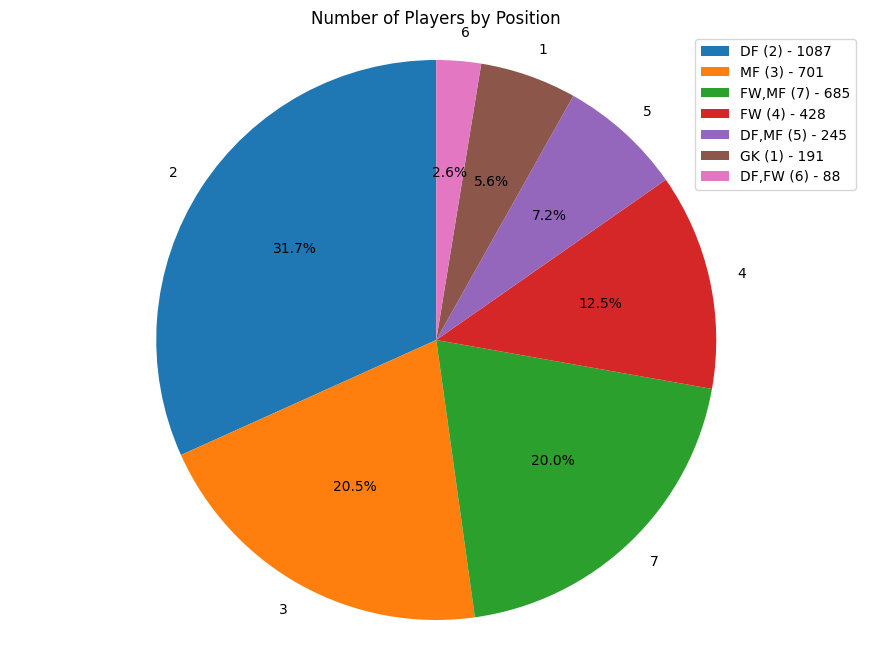
\includegraphics[scale=0.5]{players_by_position.png}
    \caption{Liczba piłkarzy na danej pozycji}
    \label{img:photo1}
\end{figure}

Powyższy diagram przedstawia liczbę piłkarzy grających na danej pozycji. Jak widać niektórzy zawodnicy grają jednocześnie na różnych pozycjach. Najwięcej w danych treningowych mamy informacji dotyczących obrońców (1087), zaś najmniej – obrońców/atakujących (88).

\begin{figure}[H]
    \centering
    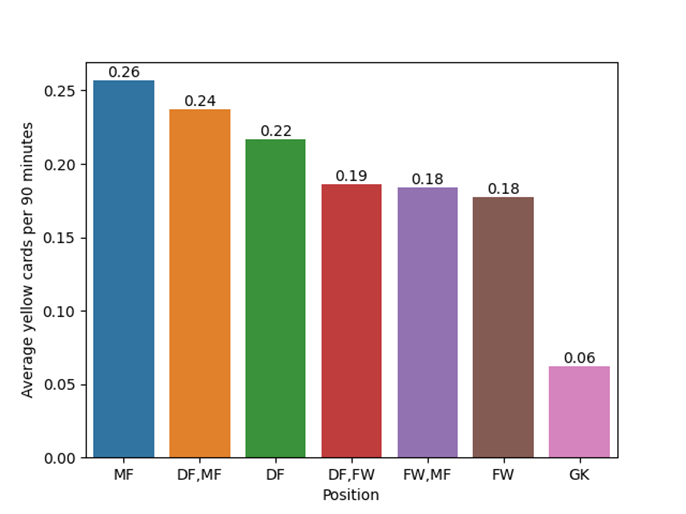
\includegraphics[scale=1.25]{avg_yellow_crd_90_by_position.png}
    \caption{Średnia liczba żółtych kartek na 90 minut na danej pozycji}
    \label{img:photo2}
\end{figure}

Powyższy diagram przedstawia średnią liczbę żółtych kartek na 90 minut zdobytych przez zawodników na konkretnych pozycjach. Jak widać średnio na 90 minut najwięcej żółtych kartek otrzymują pomocnicy (0.26 kartki/90min), zaś najmniej – bramkarze (0.06 kartki/90min).

\begin{figure}[H]
    \centering
    \subfigure[Średnia kartek na 90 minut na danej pozycji zawodników, który rozegrali powyżej 30 meczy]{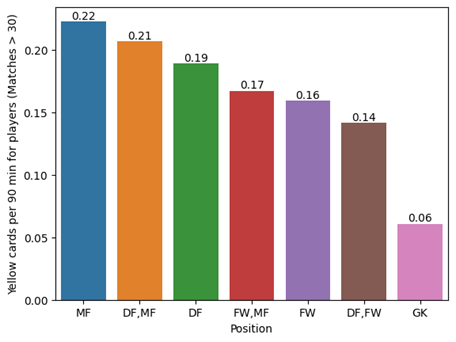
\includegraphics[width=0.4\textwidth]{avg_yellow_crd_90_by_position_MP30.png}}
    \hfill
    \subfigure[Średnia kartek na 90 minut na danej pozycji zawodników, który rozegrali poniżej 20 meczy]{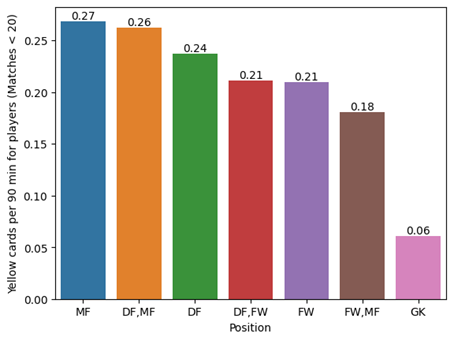
\includegraphics[width=0.4\textwidth]{avg_yellow_crd_90_by_position_MP20.png}}
\end{figure}

Powyższe porównanie przedstawia średnią liczbę żółtych kartek na 90 minut zdobytych przez zawodników na konkretnych pozycjach przy określonej liczbie rozegranych meczów. Można zauważyć, że zawodnicy, którzy rozegrali więcej meczy, zdobyli stosunkowo mniej żółtych kartek na rozegrane 90 minut. Być może jest to spowodowane większym rozłożeniem się zdobytych żółtych kartek w liczbie rozegranych minut na boisku.


\begin{table}[H]
    \centering
    \begin{tabular}{|c|c|c|c|c|}
    \hline
    Lp. & Player & Position & Club & YellowCardsPer90 \\
    \hline
    1 & Béni Makouana & 7 & montpellier & 1.111111 \\ \hline
    2 & Nikola Kalinić & 4 & hellas verona & 1.111111 \\ \hline
    3 & Aleksandar Sedlar & 5 & mallorca & 1.111111 \\ \hline
    4 & Kevin-Prince Boateng & 7 & hertha bsc & 1.038961 \\ \hline
    5 & David Tavares & 3 & famalicao & 1.000000 \\
    \hline
    \end{tabular}
    \caption{Top 5 piłkarzy z największą ilością żółtych kartek na 90 minut}
\end{table}

Powyższa tabela przedstawia 5 zawodników z największą liczbą zdobywanych żółtych kartek na rozegrane 90 minut. ‘’Najlepsi” zawodnicy średnio  zdobywali ponad 1 żółtą co każdy rozegrany pełny mecz.

\begin{table}[H]
    \centering
    \begin{tabular}{|c|c|c|c|c|}
    \hline
    Lp. & Player & Position & Club & FoulsPer90 \\
    \hline
    1 & Yan Brice Eteki & 4 & granada & 4.736842 \\ \hline
    2 & Tom Eaves & 4 & hull city & 4.214286 \\ \hline
    3 & Martin Adeline & 7 & reims & 4.102564 \\ \hline
    4 & Julio Romão & 5 & santa clara & 4.000000 \\ \hline
    5 & Monchu & 3 & granada & 3.918919 \\
    \hline
    \end{tabular}
    \caption{Top 5 piłkarzy z największą ilością fauli na 90 minut}
\end{table}

Powyższa tabela przedstawia 5 zawodników z największą liczbą popełnionych fauli na mecz. Co ciekawe, żaden z zawodnik nie widnieje w obydwóch tabelach.

\begin{figure}[H]
    \centering
    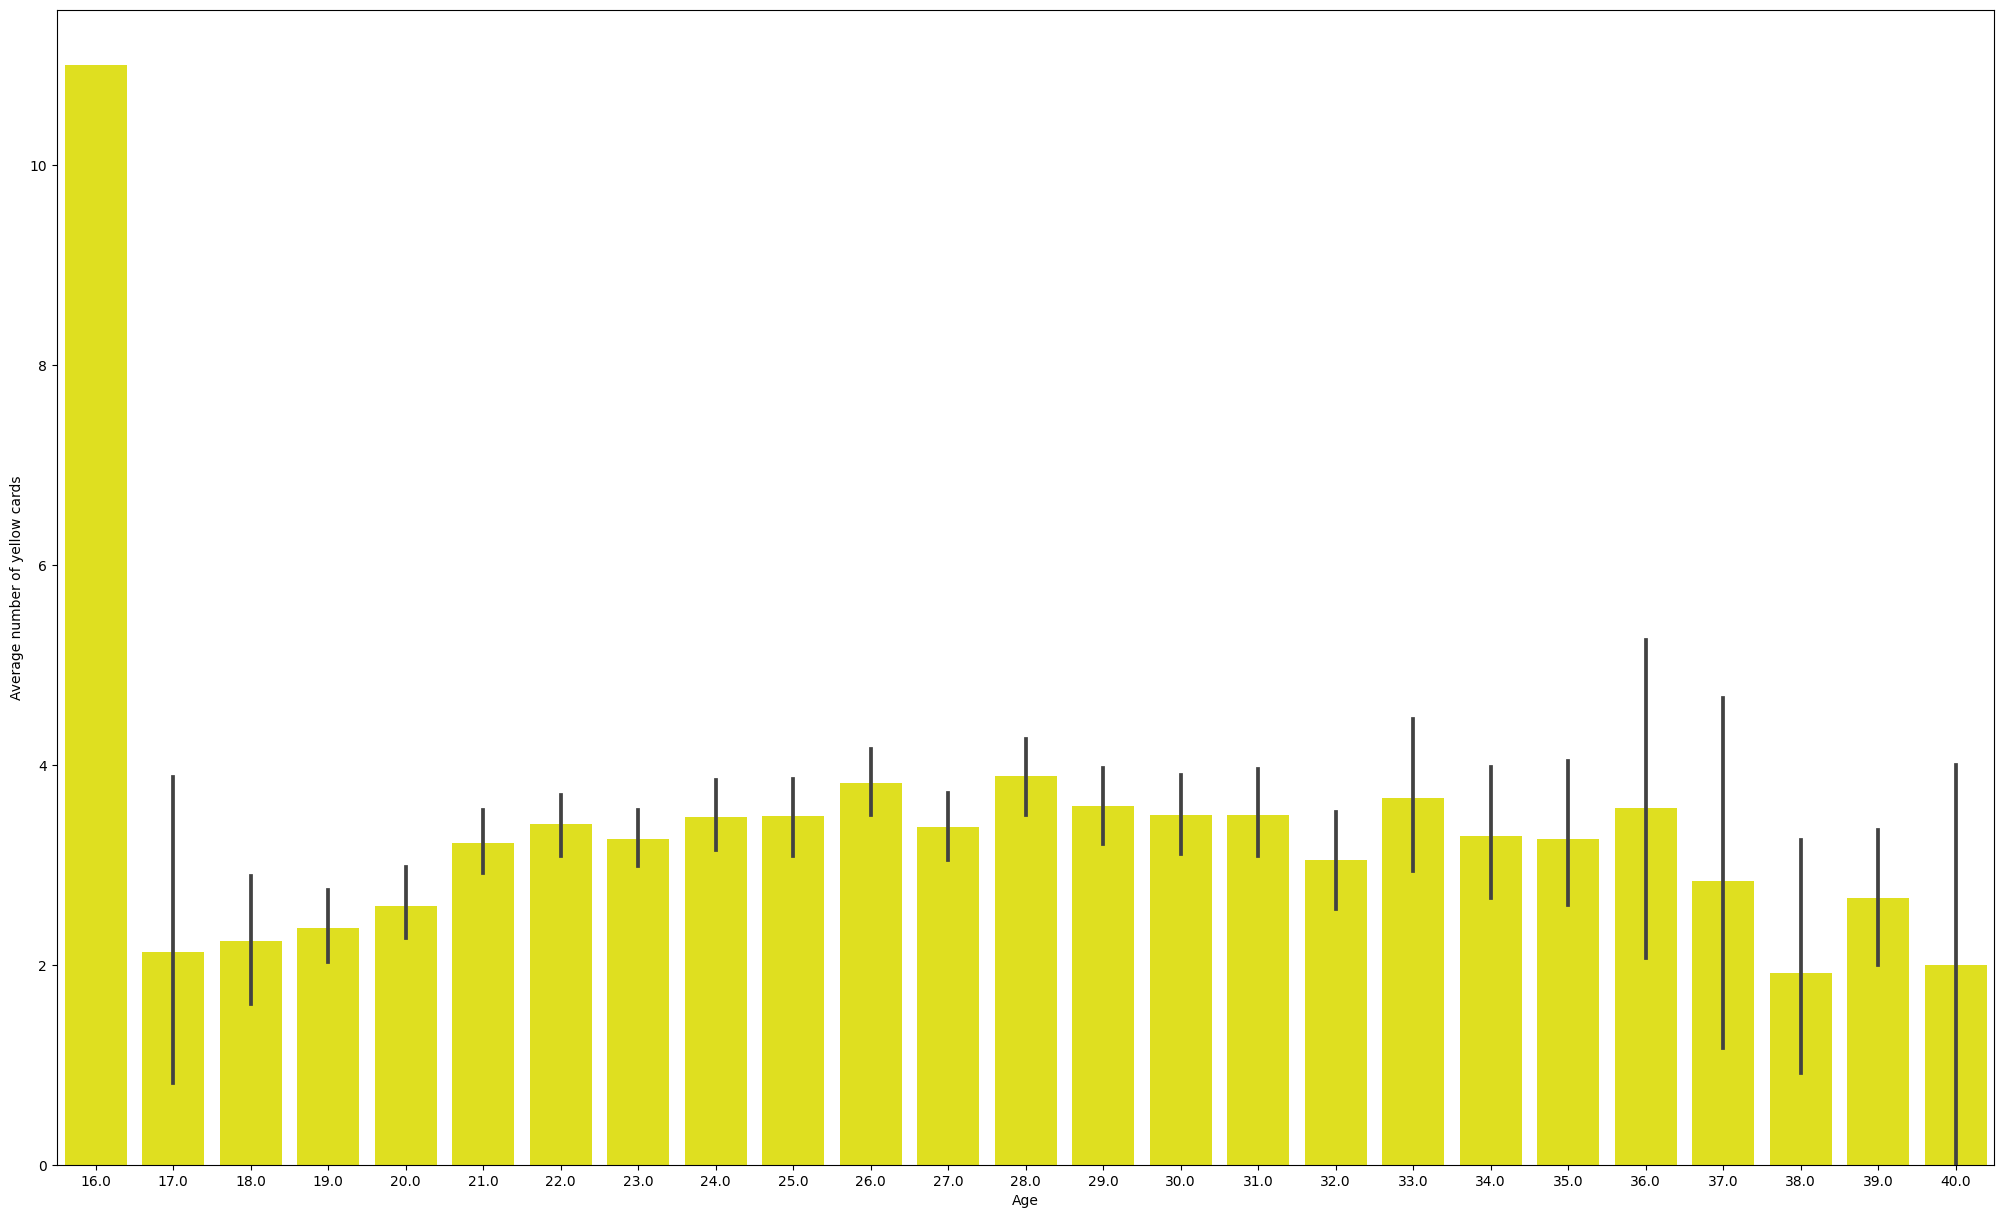
\includegraphics[scale=0.2]{yellow_cards_by_age.png}
    \caption{Średnia liczba żółtych kartek dla danego wieku piłkarzy}
    \label{img:photo3}
\end{figure}

Powyższy diagram przedstawia średnią liczbę zdobytych żółtych kartek w sezonie przez zawodników pogrupowanych według wieku. Jak widać, słupek diagramu dla 16-latków znacznie przewyższa pozostałe. Jest to pewnie spowodowane małą liczbą zawodników w tym wieku i dużą liczbą kartek jednego zawodnika. Pionowe kreski oznaczają odchylenie standardowe dla danej grupy wiekowej i można zauważyć, że dla 16-letnich zawodników ta kreska jest praktycznie nie widoczna, co mogłoby potwierdzać moje wcześniejsze wytłumaczenie. Odchylenie standardowe dla najstarszych zawodników jest widocznie większe, co świadczy o dużej rozbieżności w kwestii zdobytej liczby żółtych kartek.

\begin{figure}[H]
    \centering
    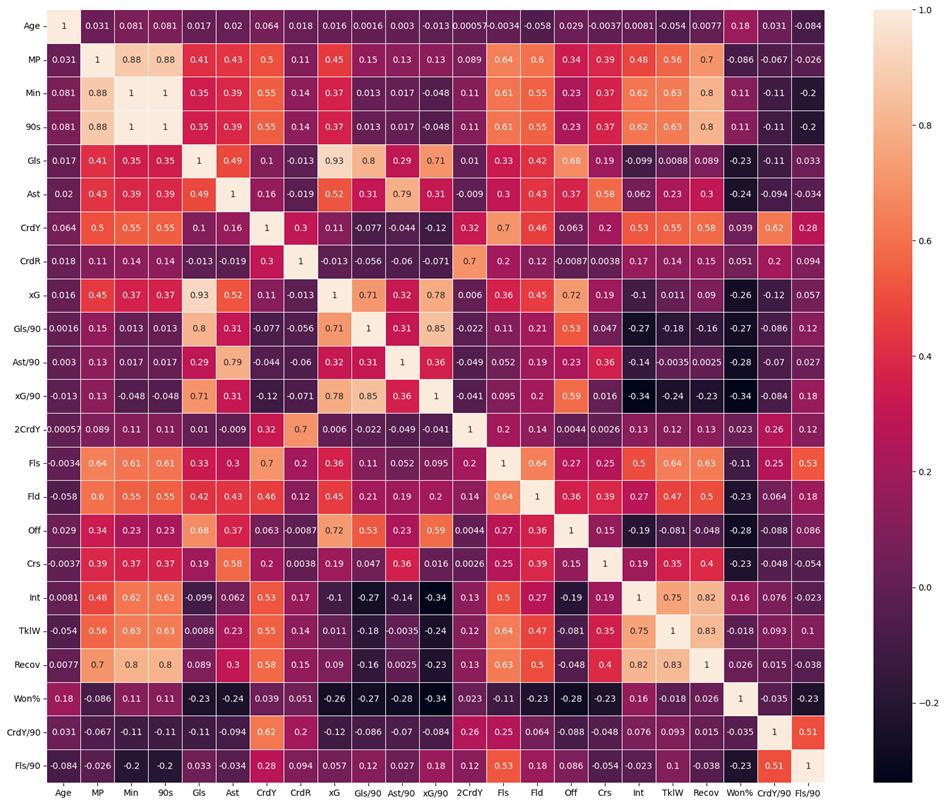
\includegraphics[scale=0.95]{correlation_matrix.png}
    \caption{Macierz korelacji statystyk piłkarzy}
    \label{img:photo4}
\end{figure}

Ostatni w tej sekcji diagram przedstawia macierz współczynników korelacji pomiędzy poszczególnymi statystykami piłkarzy. Im jaśniejszy jest kwadrat, tym większa dodatnia korelacja. Im ciemniejszy jest kwadrat, tym większa ujemna korelacja.

Można dostrzec kilka bloków atrybutów, które wskazują na korelację pomiędzy sobą np. blok dotycząca oczekiwanych goli i asyst czy rozegranych minut i meczy. Niestety dla atrybutu żółtych kartek trudno odnotować jakieś znaczące zależności.

\newpage
\section{Trenowanie i testowanie modeli regresji}

\subsection{Krótkie omówienie}

Moje obliczenia zostały podzielone na 2 części. Pierwsza część dotyczy przewidzenia liczby żółtych kartek zdobytych na 90 minut przez zawodników, zaś druga część skupia się na przewidzeniu całkowitej liczby żółtych kartek w sezonie, na podstawie statystyk piłkarzy.

\subsection{Modele}

Aby maksymalnie wykorzystać potencjał, do moich obliczeń wykorzystałem następujące modele \footnote{więcej informacji dotyczących modeli i indywidualnych parametrów użytych w obliczeniach zostały przedstawione w notebook’u z obliczeniami notebook.py}:

\begin{itemize}
    \item LinearRegression z biblioteki sklearn
    \item XGBRegressor z biblioteki xgboost
    \item LGBMRegressor z biblioteki lightgbm
    \item Neural Networks z biblioteki keras
    \item DecisionTreeRegressor z biblioteki sklearn
\end{itemize}

\subsubsection{LinearRegression}
Model LinearRegression jest podstawowym modelem regresji liniowej, który stara się znaleźć najlepsze dopasowanie liniowe między zależną zmienną a zestawem niezależnych zmiennych. Wykorzystuje metodę najmniejszych kwadratów, aby minimalizować różnicę między rzeczywistymi a przewidywanymi wartościami.

\subsubsection{XGBRegressor}
Model XGBRegressor to implementacja algorytmu gradient boosting zespołowego (gradient boosting machine) opartego na drzewach decyzyjnych. Wykorzystuje technikę wzmacniania gradientowego, gdzie iteracyjnie dodaje drzewa decyzyjne, minimalizując gradient funkcji straty. Ten model jest znany ze swojej wysokiej wydajności i zdolności do radzenia sobie z dużymi i złożonymi zbiorami danych.

\subsubsection{LGBMRegressor}
Model LGBMRegressor to kolejna implementacja gradient boosting zespołowego, która wykorzystuje drzewa decyzyjne z optymalizacją na podstawie histogramu. Działa na podobnej zasadzie jak XGBRegressor, ale zastosowana technika optymalizacji pozwala na szybsze trenowanie modelu i wykorzystanie mniej zasobów obliczeniowych.

\subsubsection{Sieci neuronowe}

Modele sieci neuronowych pozwalają na tworzenie różnych architektur sieci neuronowych, które są zdolne do uczenia się nieliniowych zależności i są często stosowane w zadaniach regresji, gdzie zależności są bardziej skomplikowane.

\subsubsection{DecisionTreeRegressor}
DecisionTreeRegressor jest modelem regresji opartym na drzewie decyzyjnym. Drzewo decyzyjne to struktura hierarchiczna, w której każdy węzeł reprezentuje test na jednej z cech, a każda gałąź odpowiada różnym wynikom testu. Drzewo jest trenowane na podstawie danych treningowych, gdzie cechy są używane do podziału danych na kolejne węzły, a liście drzewa zawierają przewidywane wartości regresyjne.

\vspace{0.5cm} 
\noindent Podczas tworzenia wybranych modeli zastosowano metodę GridSearch do optymalizacji hiperparametrów.

\subsection{Cechy}

W pierwszej części, aby dokonać predykcji liczby żółtych kartek na 90 minut wykorzystano następujące cechy piłkarzy:

\begin{itemize}
  \item wiek
  \item liczba fauli na 90 minut
  \item liczba rozegranych 90 minut
  \item liczba goli na 90 minut
  \item liczba wślizgów
  \item liczba przechwytów
\end{itemize}

\noindent W drugiej części do przewidzenia liczby żółtych kartek w sezonie użyto poniższych statystyk:

\begin{itemize}
  \item pozycja zawodnika
  \item całkowita liczba rozegranych minut w sezonie
  \item całkowita liczba fauli w sezonie
  \item całkowita liczba wymuszonych fauli na przeciwniku w sezonie
  \item całkowita liczba wślizgów w sezonie
  \item całkowita liczba przechwytów w sezonie
  \item całkowita liczba odzyskanych piłek
\end{itemize}

\subsection{Analiza obliczeń i wyników}

Zacznijmy omówienie pierwszej części analizy, w ramach której na początku dokonano wyboru najlepszego stopnia wielomianu dla moich modelów regresji na najprostszym modelu regresji – LinearRegression. Do przetestowania modelu i sprawdzenia $r^2$ wykorzystano zarówno dane testowe, jaki i dane treningowe. 

Oto wyniki\footnote{wyniki zostały zaokrąglone do 5 miejsc po przecinku}:

\begin{table}[H]
\centering
\begin{tabular}{|c|c|c|}
\hline
Stopień wielomianu & Treningowe $r^2$ & Testowe $r^2$ \\
\hline
2 & 0.30666 & 0.30121 \\ \hline
3 & 0.32247 & 0.29423 \\ \hline
4 & 0.35218 & 0.28817 \\ \hline
5 & 0.40251 & 0.15600 \\ \hline
6 & 0.44912 & -16.68713 \\ \hline
7 & 0.58093 & -505.44356 \\ \hline
8 & 0.71442 & -101212.57251 \\ 
\hline
\end{tabular}
\caption{Tabela wyników modelu}
\end{table}


Jak widać, im wyższy stopień wielomianu, tym lepsze dopasowanie modelu do wykorzystanych danych treningowych, lecz wraz ze wzrostem, drastycznie maleje $r^2$ dla danych testowych, co nie jest dobrą oznaką. Z tego też powodu została podjęta decyzja, aby wykorzystać domyślny wielomian - stopnia drugiego - gdyż daje porównywalne wyniki dla danych treningowych i testowych, co może pomóc znaleźć odpowiedni model oraz rezultat.

\newpage
Poniżej przedstawiono wyniki wykorzystanych w obliczeniach modeli
\vspace{0.5cm}

Szczegółowe wyniki dla LinearRegression:
\vspace{0.5cm}

Wielomian:
$y = 0.00301918x_1 + 0.12637597x_2 - 0.00132616x_3 - 0.11237664x_4 - 0.00019764x_5 + 0.00118643x_6 - 0.00259398$, gdzie:

\begin{itemize}[label={}, leftmargin=*]
  \item $y$ -- przewidywana liczba żółtych kartek na 90 minut (\textit{CrdY/90})
  \item $x_1$ -- wiek piłkarza (\textit{Age})
  \item $x_2$ -- liczba fauli na 90 minut (\textit{Fls/90})
  \item $x_3$ -- liczba rozegranych 90 minut (\textit{90s})
  \item $x_4$ -- liczba goli na 90 minut (\textit{Gls/90})
  \item $x_5$ -- liczba wślizgów (\textit{TklW})
  \item $x_6$ -- liczba przechwytów (\textit{Int})
\end{itemize}

W ramach wyjaśnienia moich wyników, poniżej przedstawiono statystyki, które zostały obliczone w celu określenia jakości rezultatów modelu.

$r^2$ (ang. r-squared) jest miarą jakości dopasowania modelu regresji do danych. Oznacza ono współczynnik determinacji i jest liczbową wartością między 0 a 1. Wyższa wartość $r^2$ wskazuje na lepsze dopasowanie modelu do danych.
 
MAE (ang. mean absolute error) to miara błędu średniego bezwzględnego w modelach regresji. Mierzy ona przeciętną różnicę między prognozowanymi wartościami modelu a rzeczywistymi wartościami danych.

MAE oblicza się poprzez zsumowanie wartości bezwzględnych różnic między prognozami a rzeczywistymi wartościami, a następnie podzielenie przez liczbę przykładów danych. Jest to miara bezwzględna, co oznacza, że nie bierze pod uwagę kierunku ani znaku błędu.

MSE (ang. mean squared error) to miara błędu średniokwadratowego w modelach regresji. Jest to jedna z najczęściej stosowanych miar błędu, która mierzy średnią kwadratową różnicę między prognozowanymi wartościami modelu a rzeczywistymi wartościami danych.

MSE oblicza się poprzez zsumowanie kwadratów różnic między prognozami a rzeczywistymi wartościami, a następnie podzielenie przez liczbę przykładów danych. Kwadratowa natura miary powoduje, że większe błędy mają większy wpływ na wynik niż mniejsze błędy.


Poniżej przedstawiono wyniki obliczeń predykcji liczby żółtych kartek na 90 minut \footnote{wyniki zostały podane z dokładnością do 5 miejsc po przecinku}:

\begin{table}[H]
\centering
\begin{tabular}{|c|c|c|c|c|}
\hline
Model & Rodzaj danych & $r^2$ & MAE & MSE \\ \hline
\cline{2-5}
LinearRegression & treningowe & 0.29130 & 0.10077 & 0.01834 \\
\cline{2-5}
& testowe & 0.32254 & 0.09300 & 0.01524 \\
\hline
XGBRegression & treningowe & 0.88237 & 0.04053 & 0.00304 \\
\cline{2-5}
& testowe & 0.22403 & 0.09968 & 0.01746 \\
\hline
LGBMRegressor 1 & treningowe & 0.63725 & 0.07475 & 0.00939 \\
\cline{2-5}
& testowe & 0.27425 & 0.09503 & 0.01633 \\
\hline
LGBMRegressor 2 & treningowe & 0.71037 & 0.06583 & 0.00750 \\
\cline{2-5}
& testowe & 0.26028 & 0.09650 & 0.01664 \\
\hline
NN Keras 1 & treningowe & 0.31578 & 0.09483 & 0.01771 \\
\cline{2-5}
& testowe & 0.28987 & 0.09323 & 0.01598 \\
\hline
NN Keras 2 & treningowe & 0.27414 & 0.09976 & 0.01879 \\
\cline{2-5}
& testowe & 0.30203 & 0.09385 & 0.01571 \\
\hline
DecisionTreeRegressor 1 & treningowe & 0.99999 & 0.00001 & 0.00000 \\
\cline{2-5}
& testowe & -0.42458 & 0.13245 & 0.03205 \\
\hline
DecisionTreeRegressor 2 & treningowe & 0.34142 & 0.09737 & 0.01705 \\
\cline{2-5}
& testowe & 0.28730 & 0.09538 & 0.01604 \\
\hline
\end{tabular}
\caption{Wyniki dla wytrenowanych modelach dla liczby żółtych kartek na 90 minut}
\end{table}

\begin{figure}[H]
  \centering
  \begin{minipage}[b]{0.5\textwidth}
    \centering
    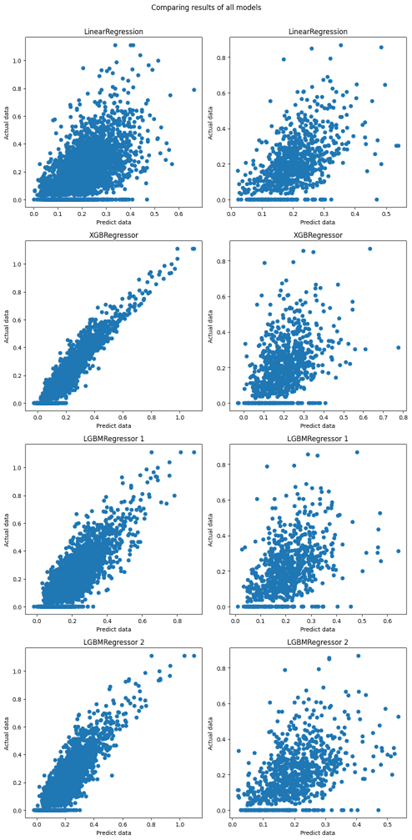
\includegraphics[width=\textwidth]{all_models_1.png}
    % \caption{Podpis do pierwszego obrazu}
    \label{fig:obraz1}
  \end{minipage}%
  \begin{minipage}[b]{0.5\textwidth}
    \centering
    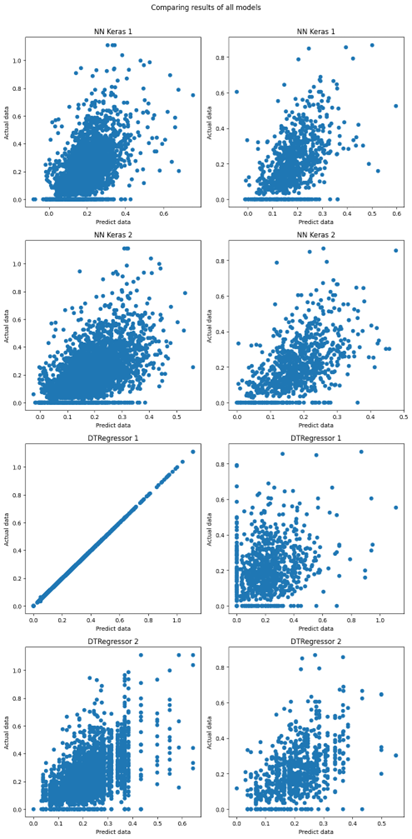
\includegraphics[width=\textwidth]{all_models_2.png}
    % \caption{Podpis do drugiego obrazu}
    \label{fig:obraz2}
  \end{minipage}
  \captionsetup{justification=centering}
  \caption{Porównanie wyników wszystkich modeli z rzeczywistymi wartościami liczb żółtych kartek na 90 minut}
  \label{fig:all_models1}
\end{figure}

Ze względu na to, że niemożliwe jest zwizualizowanie sensownego wykresu dla więcej niż 3 zmiennych, dla każdego wykorzystanego modelu, przedstawiono wykresy (\ref{fig:all_models1}) (\ref{fig:all_models2}) porównujące wyniki przewidziane przez modele z tymi prawdziwymi. 

\newpage
Przechodząc do drugiej części analizy, w tej części dokonano prób przewidzenia całkowitej liczby zdobytych żółtych kartek przez zawodników w ciągu całego sezonu. Poniżej przedstawiono wyniki wykorzystanych w obliczeniach modeli.
\vspace{0.5cm}

Szczegółowe wyniki dla LinearRegression:
\vspace{0.5cm}

Wielomian:
$y = -0.13721626x_1 + 0.00021294x_2 - 0.11574336x_3  + 0.00635061x_4 - 0.03066969x_5 - 0.00127684x_6 + 0.00028151x_7 + 0.6805319$, gdzie:

\begin{itemize}[label={}, leftmargin=*]
  \item $y$ - przewidywana liczba żółtych kartek na 90 minut (\textit{CrdY})
  \item $x_1$ - pozycja piłkarza (\textit{Pos})
  \item $x_2$ - całkowita liczba rozegranych minut w sezonie  (\textit{Min})
  \item $x_3$ - całkowita liczba fauli w sezonie  (\textit{Fls})
  \item $x_4$ - całkowita liczba wymuszonych fauli na przeciwniku w sezonie  (\textit{Fld})
  \item $x_5$ - całkowita liczba wślizgów w sezonie  (\textit{Int})
  \item $x_6$ - całkowita liczba przechwytów w sezonie  (\textit{TklW})
  \item $x_7$ - całkowita liczba odzyskanych piłek  (\textit{Recov})
\end{itemize}

\begin{table}[H]
\centering
\begin{tabular}{|c|c|c|c|c|}
\hline
Model & Rodzaj danych & $r^2$ & MAE & MSE \\ \hline
\cline{2-5}
LinearRegression & treningowe & 0.54764 & 1.42172 & 3.54680 \\
\cline{2-5}
& testowe & 0.55612 & 1.33010 & 3.17087 \\
\hline
XGBRegression & treningowe & 0.93801 & 0.51401 & 0.48607 \\
\cline{2-5}
& testowe & 0.47386 & 1.44746 & 3.75851 \\
\hline
LGBMRegressor 1 & treningowe & 0.78350 & 1.02103 & 1.69751 \\
\cline{2-5}
& testowe & 0.50768 & 1.40121 & 3.51693 \\
\hline
LGBMRegressor 2 & treningowe & 0.82180 & 0.90995 & 1.39723 \\
\cline{2-5}
& testowe & 0.50022 & 1.40728 & 3.57020 \\
\hline
NN Keras 1 & treningowe & 0.55575 & 1.38079 & 3.48326 \\
\cline{2-5}
& testowe & 0.54628 & 1.32588 & 3.24114 \\
\hline
NN Keras 2 & treningowe & 0.54081 & 1.41273 & 3.60038 \\
\cline{2-5}
& testowe & 0.54745 & 1.32389 & 3.23279 \\
\hline
DecisionTreeRegressor 1 & treningowe & 1.00000 & 0.00000 & 0.00000 \\
\cline{2-5}
& testowe & -0.01841 & 2.01841 & 7.27503 \\
\hline
DecisionTreeRegressor 2 & treningowe & 0.56931 & 1.39571 & 3.37695 \\
\cline{2-5}
& testowe & 0.54138 & 1.36877 & 3.27620 \\
\hline
\end{tabular}
\caption{Wyniki dla wytrenowanych modelach dla całkowitej liczby żółtych kartek w sezonie}
\end{table}

\begin{figure}[H]
  \centering
  \begin{minipage}[b]{0.5\textwidth}
    \centering
    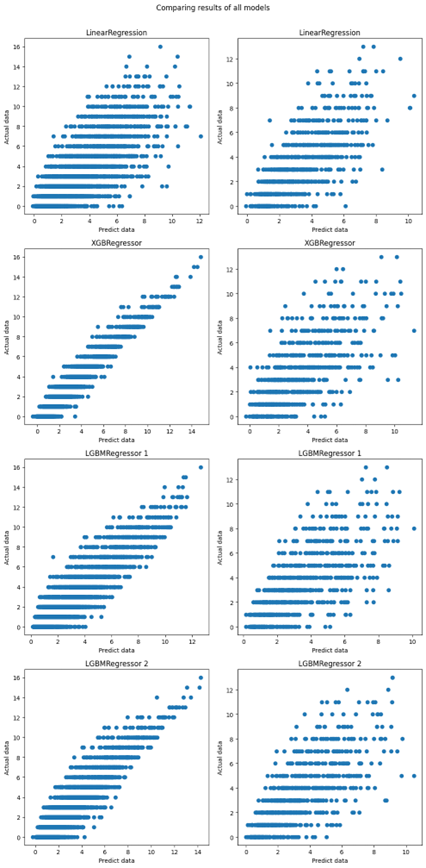
\includegraphics[width=\textwidth]{all_models_3.png}
    % \caption{Podpis do pierwszego obrazu}
    \label{fig:obraz3}
  \end{minipage}%
  \begin{minipage}[b]{0.5\textwidth}
    \centering
    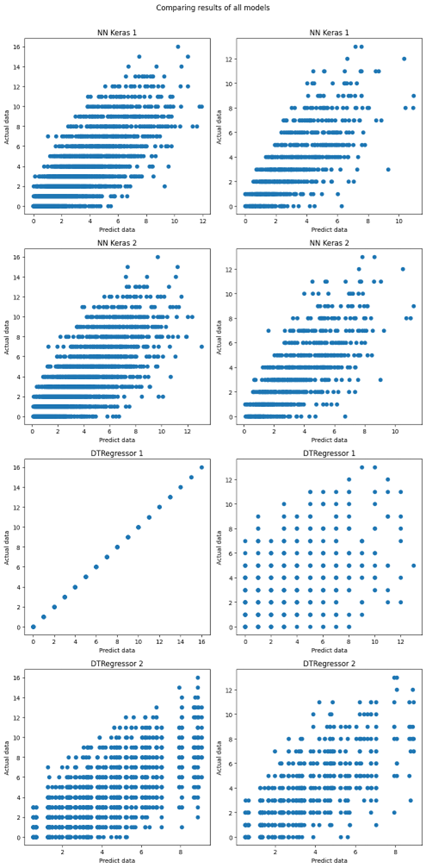
\includegraphics[width=\textwidth]{all_models_4.png}
    % \caption{Podpis do drugiego obrazu}
    \label{fig:obraz4}
  \end{minipage}
  \captionsetup{justification=centering}
  \caption{Porównanie wyników wszystkich modeli z rzeczywistymi wartościami liczb żółtych kartek zdobytych w całym sezonie}
  \label{fig:all_models2}
\end{figure}

\newpage
\subsection{Porównanie badań i ich rezultatów}

W pierwszej części badania wykazały, że żółte kartki są nie do końca przewidywalne i trudno jest je przewidzieć. Dokonując predykcji liczby żółtych kartek na 90 minut, modele nie poradziły sobie najlepiej.

\begin{figure}[H]
  \centering
  \begin{minipage}[b]{0.5\textwidth}
    \centering
    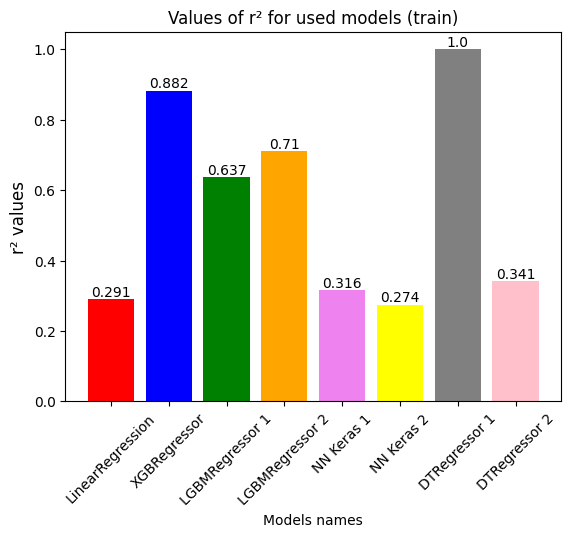
\includegraphics[width=\textwidth]{all_r2_1.png}
    % \caption{Podpis do pierwszego obrazu}
    \label{fig:all_r2_train1}
  \end{minipage}%
  \begin{minipage}[b]{0.5\textwidth}
    \centering
    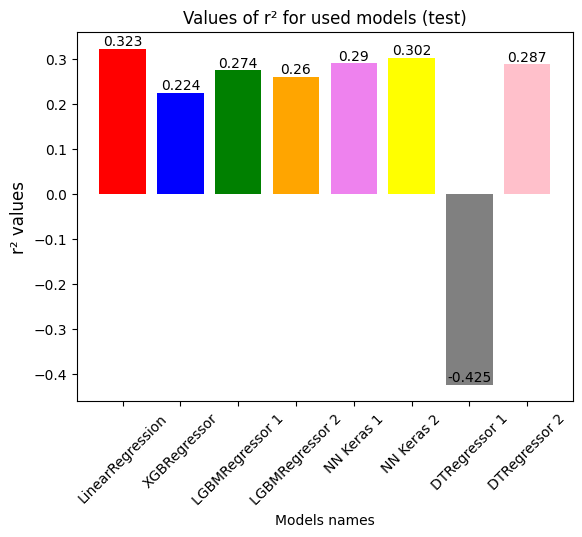
\includegraphics[width=\textwidth]{all_r2_2.png}
    % \caption{Podpis do drugiego obrazu}
    \label{fig:all_r2_test1}
  \end{minipage}
  \captionsetup{justification=centering}
  \caption{Porównanie $r^2$ dla danych treningowych i testowych dla liczby żółtych kartek na 90 minut}
  \label{fig:all_r2_1}
\end{figure}

Jak widać powyżej, mimo bardzo dobrego dopasowania się modeli XGBRegressor (0.882) oraz domyślnego DecisionTreeRegressor (aż 1.0) do danych treningowych, tak dla danych testowych okazały się najgorsze – DecisionTreeRegressor uzyskał nawet ujemny współczynnik $r^2$  na poziomie -0.513, co oznacza, że model jest gorszy niż model, który po prostu przewiduje średnią wartość kartek.

Pozostałe modele dla danych treningowych poradziły sobie nienajlepiej. Co jest warte uwagi, to to, że model klasycznej regresji liniowej – LinearRegression – poradził sobie tak samo zarówno dla danych treningowych, jak i testowych. Ponadto model sieci neuronowych z warunkiem stopu mimo, że dla danych treningowych poradził sobie gorzej od klasycznego, to dla danych testowych poradził sobie nieznacznie lepiej.

Jak wiadomo, mimo że $r^2$ pokazuje poziomo dopasowania wartości, tak nie jest jedyną miarą jakości modeli. Przejdźmy zatem do tego, jak wyglądają błędy modeli – MAE i MSE.

\begin{figure}[H]
  \centering
  \begin{minipage}[b]{0.5\textwidth}
    \centering
    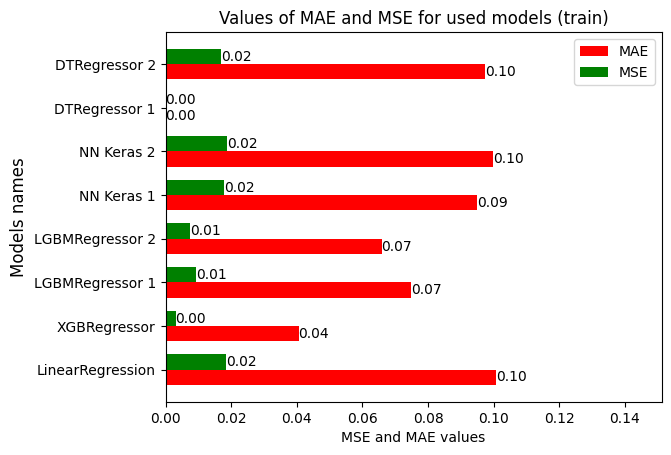
\includegraphics[width=\textwidth]{all_errors_1.png}
    % \caption{Podpis do pierwszego obrazu}
    \label{fig:all_errors_1}
  \end{minipage}%
  \begin{minipage}[b]{0.5\textwidth}
    \centering
    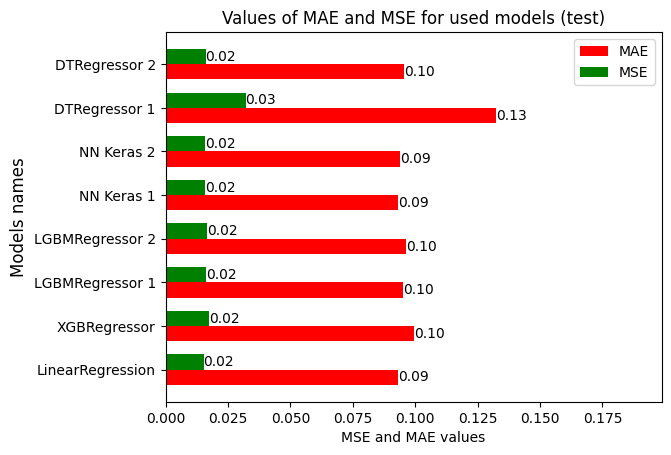
\includegraphics[width=\textwidth]{all_errors_2.png}
    % \caption{Podpis do drugiego obrazu}
    \label{fig:all_errors_2}
  \end{minipage}
  \captionsetup{justification=centering}
  \caption{Porównanie MAE i MSE dla danych treningowych i testowych dla liczby żółtych kartek na 90 minut}
  \label{fig:all_errors_1_1}
\end{figure}

\begin{figure}[H]
  \centering
  \begin{minipage}[b]{0.5\textwidth}
    \centering
    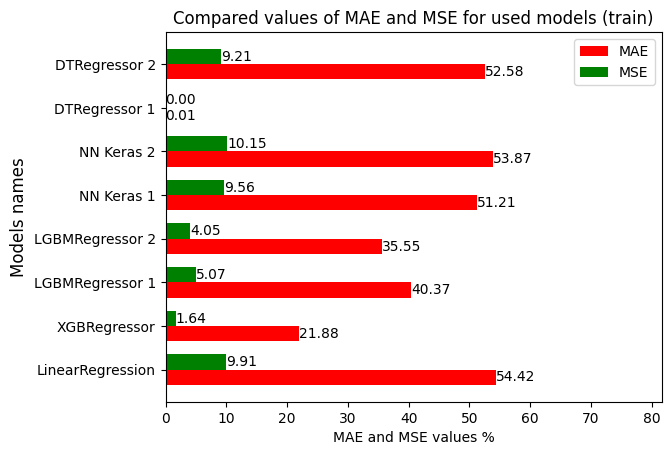
\includegraphics[width=\textwidth]{all_errors_3.png}
    % \caption{Podpis do pierwszego obrazu}
    \label{fig:all_errors_3}
  \end{minipage}%
  \begin{minipage}[b]{0.5\textwidth}
    \centering
    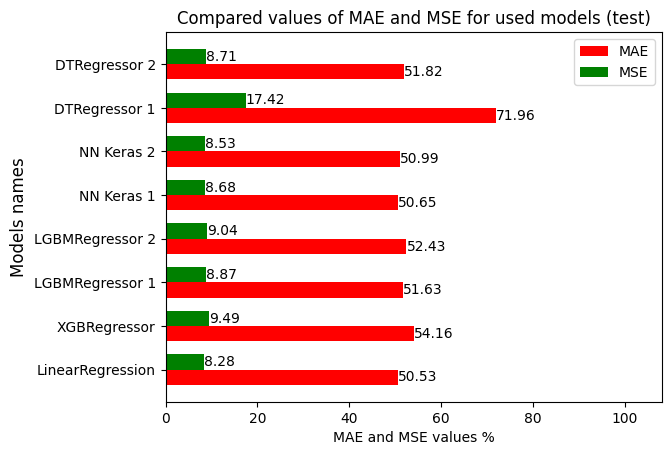
\includegraphics[width=\textwidth]{all_errors_4.png}
    % \caption{Podpis do drugiego obrazu}
    \label{fig:all_errors_4}
  \end{minipage}
  \captionsetup{justification=centering}
  \caption{Porówanie wartości MAE i MSE porównanych do mediany dla danych treningowych i testowych dla liczby żółtych kartek na 90 minut}
  \label{fig:all_errors_1_2}
\end{figure}


W tym przypadku MSE nie jest zbyt dobrym wyznacznikiem jakości, ze względu na to, że działamy w większości przypadkach na wartościach ułamkowych z przedziału od 0 do 1. 

Skupmy się zatem na MAE i jak widać, mimo że błąd na poziomie nie wydaje się zbyt duży, to w porównaniu do mediany równej 0.18519 spośród wszystkich liczby żółtych kartek zdobytych na 90 minut jest to duża wartość. Najmniejszy błąd procentowy dla danych testowych jest dla modelu klasycznej regresji liniowej na poziomie 50.53\% (MAE = 0.09), zaś największy dla domyślnego DecisionTreeRegressor – 71.96\% (MAE = 0.13). W przypadku gdyby piłkarz rozegrał niewiele meczy, modele zbytnio nie odbiegałyby od rzeczywistych wyników, lecz piłkarze w samej lidzie grają nawet po 40 meczów i w tym przypadku błąd byłby już znaczny – przynajmniej 3.6 kartki na sezon.
\vspace{0.5cm}

W drugiej części dokonując predykcji liczby żółtych kartek w całym sezonie, modele poprawiły swoje wyniki.

\begin{figure}[H]
  \centering
  \begin{minipage}[b]{0.5\textwidth}
    \centering
    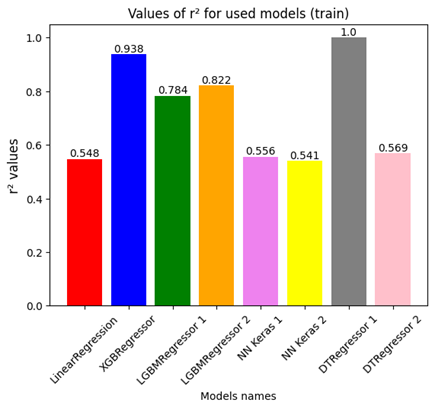
\includegraphics[width=\textwidth]{all_r2_3.png}
    % \caption{Podpis do pierwszego obrazu}
    \label{fig:all_r2_train2}
  \end{minipage}%
  \begin{minipage}[b]{0.5\textwidth}
    \centering
    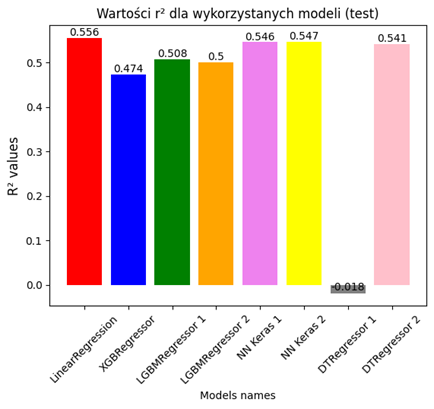
\includegraphics[width=\textwidth]{all_r2_4.png}
    % \caption{Podpis do drugiego obrazu}
    \label{fig:all_r2_test2}
  \end{minipage}
  \captionsetup{justification=centering}
  \caption{Porównanie $r^2$ dla danych treningowych i testowych dla całkowitej liczby żółtych kartek w sezonie}
  \label{fig:all_r2_2}
\end{figure}

Podobnie jak w poprzedniej części, modele XGBRegressor i domyślny DecisionTreeRegressor poradziły sobie najlepiej, odnotowując wartości $r^2$ na poziomach kolejno 0.938 oraz 1.0. Pozostałe modele też znacznie poprawiły swoje wyniki – największy wzrost w porównaniu do poprzedniej części dla danych testowych odnotowały: model XGBRegression (wzrost z poziomu 0.147 do 0.474), model sparametryzowanego DecisionTreeRegression (wzrost z poziomu 0.23 do 0.541) oraz model domyślnego DecisionTreeRegression (wzrost z -0.513 do -0.018), jednak w tym przypadku nie możemy mówić o poprawie modelu, gdyż dalej jest to wartość ujemna, zdecydowanie odbiegająca od oczekiwań. 


\begin{figure}[H]
  \centering
  \begin{minipage}[b]{0.5\textwidth}
    \centering
    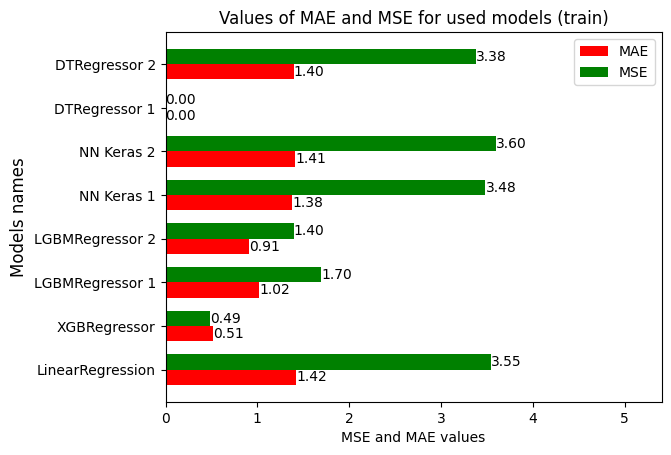
\includegraphics[width=\textwidth]{all_errors_5.png}
    % \caption{Podpis do pierwszego obrazu}
    \label{fig:all_errors_5}
  \end{minipage}%
  \begin{minipage}[b]{0.5\textwidth}
    \centering
    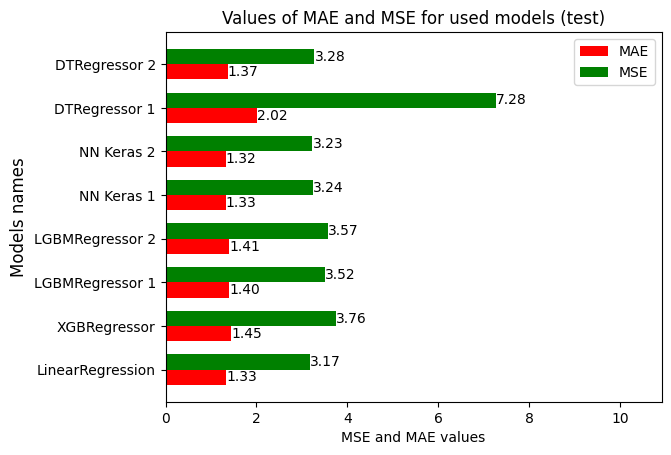
\includegraphics[width=\textwidth]{all_errors_6.png}
    % \caption{Podpis do drugiego obrazu}
    \label{fig:all_errors_6}
  \end{minipage}
  \captionsetup{justification=centering}
  \caption{Porównanie MAE i MSE dla danych treningowych i testowych dla całkowitej liczby żółtych kartek zdobytych w sezonie}
  \label{fig:all_errors_2_1}
\end{figure}

\begin{figure}[H]
  \centering
  \begin{minipage}[b]{0.5\textwidth}
    \centering
    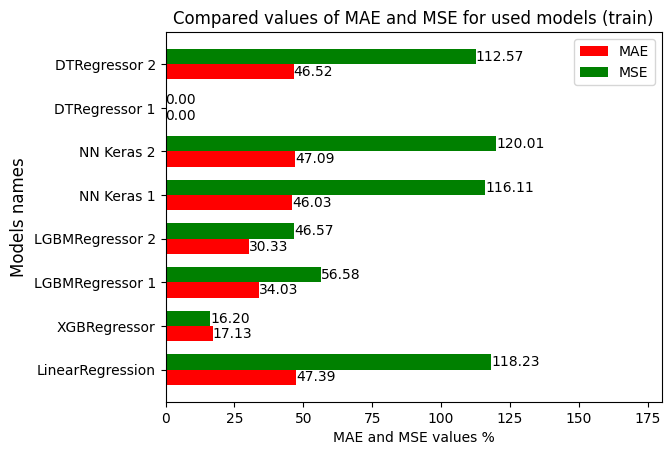
\includegraphics[width=\textwidth]{all_errors_7.png}
    % \caption{Podpis do pierwszego obrazu}
    \label{fig:all_errors_7}
  \end{minipage}%
  \begin{minipage}[b]{0.5\textwidth}
    \centering
    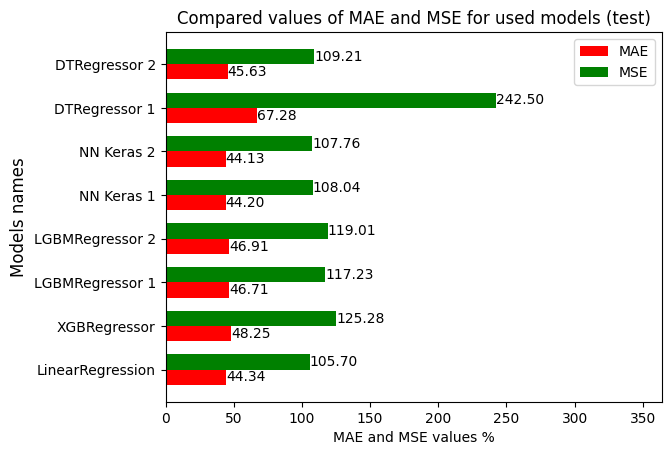
\includegraphics[width=\textwidth]{all_errors_8.png}
    % \caption{Podpis do drugiego obrazu}
    \label{fig:all_errors_8}
  \end{minipage}
  \captionsetup{justification=centering}
  \caption{Porówanie wartości MAE i MSE porównanych do mediany dla danych treningowych i testowych dla całkowitej liczby żółtych kartek zdobytych w sezonie}
  \label{fig:all_errors_2_2}
\end{figure}

Podobnie jak to było wcześniej MSE nie będzie dobrym wyznacznikiem jakości wyników wytrenowanych modeli.

Jak widać najmniejszy błąd dla danych testowych generują modele sieci neuronowych i klasycznej regresji liniowej na poziomie 1.32/1.33 kartki, co moim zdaniem nie jest najgorszym wynikiem. Zważając też na to że liczba żółtych kartek jest liczbą całkowitą, to zaokrąglając błąd, wynik błędu na poziomie 1 jest całkiem dobrym wynikiem.

Porównując to do mediany żółtych kartek wśród zawodników równej 3 kartki, można stwierdzić, że mimo wszystko modele mogłyby lepiej to przewidzieć, gdyż błąd wynosi przynajmniej 40\% wartości mediany i może wydawać się duży. 

\newpage
Sprawdźmy jeszcze, jak wygląda błąd po zaokrągleniu do najbliższej liczby całkowitej.

\begin{figure}[H]
  \centering
  \begin{minipage}[b]{0.5\textwidth}
    \centering
    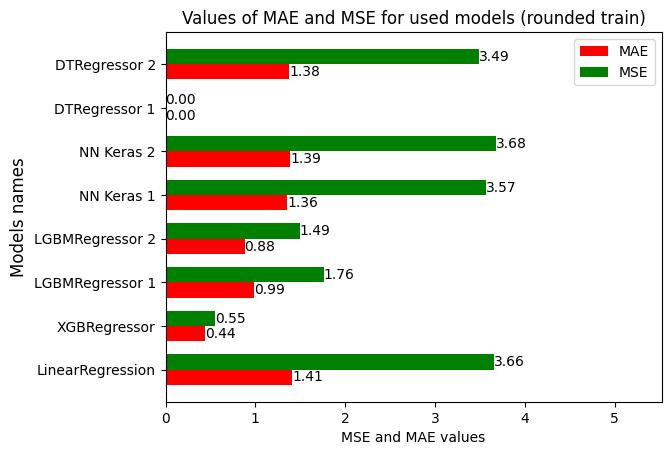
\includegraphics[width=\textwidth]{all_errors_9.png}
    % \caption{Podpis do pierwszego obrazu}
    \label{fig:all_errors_9}
  \end{minipage}%
  \begin{minipage}[b]{0.5\textwidth}
    \centering
    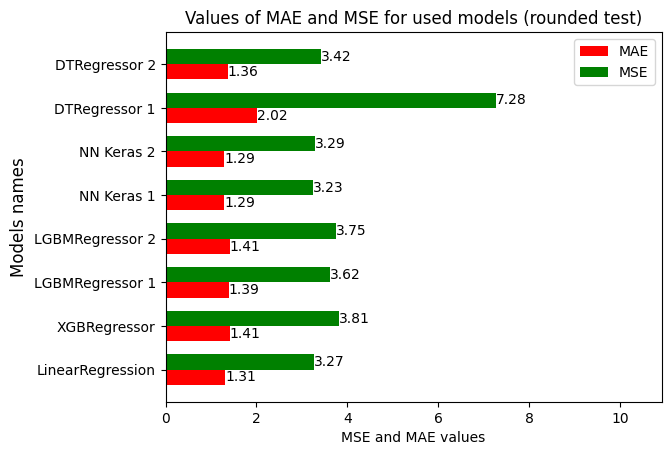
\includegraphics[width=\textwidth]{all_errors_10.png}
    % \caption{Podpis do drugiego obrazu}
    \label{fig:all_errors_10}
  \end{minipage}
  \captionsetup{justification=centering}
  \caption{Porównanie MAE i MSE dla zaokrąglonych wyników danych treningowych i testowych dla całkowitej liczby żółtych kartek zdobytych w sezonie}
  \label{fig:all_errors_3_1}
\end{figure}

\begin{figure}[H]
  \centering
  \begin{minipage}[b]{0.5\textwidth}
    \centering
    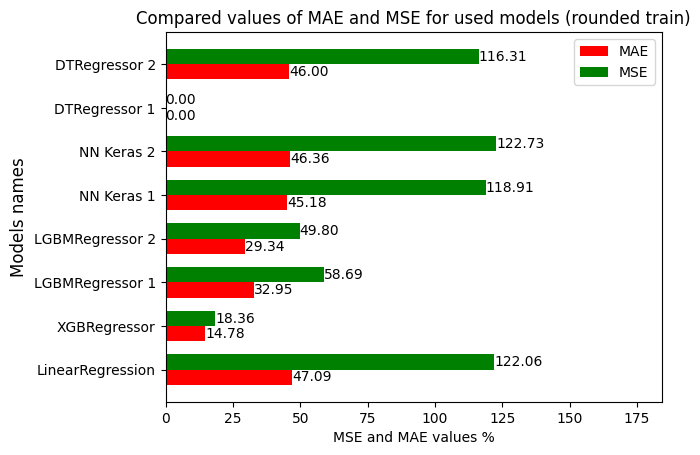
\includegraphics[width=\textwidth]{all_errors_11.png}
    % \caption{Podpis do pierwszego obrazu}
    \label{fig:all_errors_11}
  \end{minipage}%
  \begin{minipage}[b]{0.5\textwidth}
    \centering
    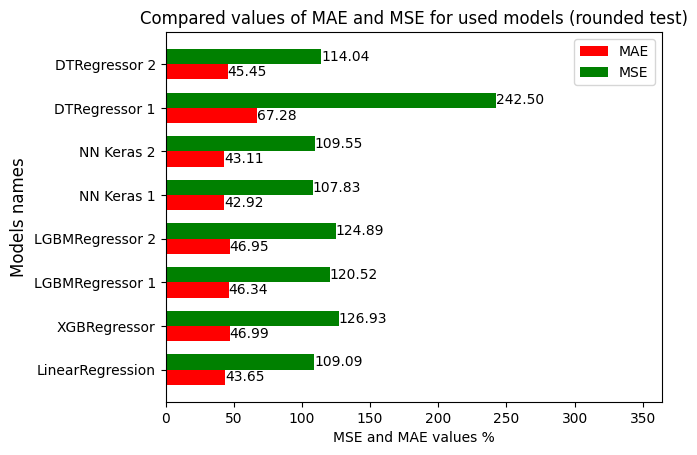
\includegraphics[width=\textwidth]{all_errors_12.png}
    % \caption{Podpis do drugiego obrazu}
    \label{fig:all_errors_12}
  \end{minipage}
  \captionsetup{justification=centering}
  \caption{Porówanie wartości MAE i MSE porównanych do mediany dla zaokrąglonych wyników danych treningowych i testowych dla całkowitej liczby żółtych kartek zdobytych w sezonie}
  \label{fig:all_errors_3_2}
\end{figure}

Jak widać statystyki nieznacznie się poprawiły, lecz zaokrąglanie i tak nie miało wielkiego wpływu na rezultaty. Najmniejszy błąd dla danych testowych po zaokrągleniu dalej mają modele sieci neuronowych oraz klasycznej regresji liniowej, kolejno 1.29 oraz 1.31. Poziom procentowy błędu w porównaniu do mediany praktycznie pozostaje bez zmian.

\newpage
\section{Wnioski}
Podsumowując obliczenia i analizę można stwierdzić, że trudno jest przewidzieć współczynnik żółtych kartek do rozegranych 90 minut. Być może jest to spowodowane zbyt dużym rozrzutem i brakiem dużej korelacji wśród statystyk na podstawie dokonano predykcji lub złym dobraniem cech. Być może wybór innych lub większej ilości statystyk mogłoby poprawić wyniki tej predykcji. Także wyniki pokazały, że długie trenowanie modelu nie pomaga i wyniki danych testowych dla takich modeli są bardzo niesatysfakcjonujące. Za przykład z pewnością można wziąć domyślny model DecisionTreeRegression, który dla danych treningowych osiągał wynik $r^2$ na perfekcyjnym poziomie 1.0, zaś dla danych testowych, jako jedyny model, osiągał $r^2$ poniżej zera, co świadczy o kompletnym braku dopasowania się do danych.

Dla predykcji całkowitej liczby żółtych kartek w całym sezonie, modele poradziły sobie w miarę dobrze, myląc się średnio o ponad jedną kartkę na cały sezon. Można też stwierdzić, że wybór cech do tej predykcji okazał się bardziej trafny i wykorzystując je w poprzedniej predykcji, można było otrzymać lepsze wyniki. Mimo że wyniki drugiej części ukazały się dla mnie zadowalające, być może użycie modeli klasyfikacji, mogłoby jeszcze poprawić wyniki, przypisując każdej wartości liczby kartek, osobną klasę.   

\vspace{0.5cm}
Podsumowując cały materiał, można stwierdzić, że statystyki meczowe zawodnika, takie jak liczba fauli czy liczba rozegranych minut, mogą mieć pewien wpływ na wystawienie żółtej kartki. Istnieje pewne prawdopodobieństwo, że zawodnik, który popełnia więcej fauli lub gra mniej minut na boisku, jest bardziej podatny na otrzymanie żółtej kartki.

Warto również pamiętać, że każdy mecz i sytuacja jest unikalna, a decyzja o wystawieniu żółtej kartki jest subiektywna i zależy od sędziego. Dlatego też, mimo analizy statystyk meczowych, przewidywanie żółtych kartek zawsze będzie obarczone pewnym stopniem niepewności.

Z pewnością dalsze analizy i badania tego problemu mają ogromny potencjał. Taka wiedza może być
niezwykle przydatna dla sztabu szkoleniowego. Przewidywanie liczby żółtych kartek może dostarczyć
informacji o tendencjach i stylu gry przeciwników oraz pomóc w opracowaniu planów gry i strategii
dla własnej drużyny. Przy zastosowaniu innych metod i strategii obliczeń, wiedza dotycząca żółtych
kartek może być niezwykle cenna w świecie piłki nożnej i w przyszłości warto poświęcić temu tematowi
więcej uwagi.



\end{document}